\documentclass{scrreprt}
\usepackage[utf8]{inputenc}
\usepackage[ngerman]{babel}
\usepackage{pslatex}
%%\setkomafont{sectioning}{\bfseries}
%%\usepackage{amsmath}
\usepackage[a4paper, left=2cm, right=2.0cm, top=2cm, bottom=2cm]{geometry}
%%\usepackage{scrpage2}
%%\clearscrheadfoot
%%\chead[-\pagemark-]{-\pagemark-} 
%%\pagestyle{scrheadings}
\usepackage{lipsum}
\linespread {1.5}
\usepackage{hyperref}
%%\usepackage{textcomp}
\usepackage{graphicx}

 
\title{W.O.R.M.}
\author{Wreck Opponents Repeatedly Meaningless}
\begin{document}
 
\maketitle
\tableofcontents
\thispagestyle{empty}
\newpage
\setcounter{page}{3}

\chapter{Einführung}
Von der populären Videospielreihe Worms inspiriert, handelt es sich bei W.O.R.M. um einen rundenbasierten, taktischen Multiplayer-Shooter. Das Ziel des Spiels ist simpel:
Zwei bis vier Spieler übernehmen die Kontrolle über jeweils drei Würmer und versuchen, sämtliche gegnerische Würmer mittels selbst ausgewählter Waffen zu eliminieren. Dabei werden Würmer zur besseren Erkennung je nach Team farblich unterschiedlich dargestellt. Treffen abgefeuerte Geschosse auf einen Wurm, erleidet dieser jedoch Schaden, unabhängig davon, ob es sich um einen Freund oder Feind handelt.
Verlieren die Würmer eines Spielers alle ihre Lebenspunkte, so scheidet dieser aus dem Spiel aus; der Gewinner ist somit derjenige, der als letztes noch Würmer kontrolliert.

Das Spiel selbst läuft so ab, dass die Spieler ihre Würmer abwechselnd in Zügen steuern. Pro Zug hat jeder Spieler 20 Sekunden lang Zeit, um einen Wurm beliebig zu bewegen und einmalig eine Waffe zu nutzen. Laufen diese 20 Sekunden ab oder wird eine Waffe verwendet, so endet die Runde des aktuellen Spielers und der nächste ist am Zug. Dieser Vorgang wird wiederholt, bis einer der Spieler das Spiel gewinnt.

\chapter{Installation und Start}
Um das Spiel nutzen zu können, ist es notwendig, Java 7 oder Java 8 zu installieren.

Eine Installation für das Spiel selbst ist nicht nötig; W.O.R.M. kann ohne weiteres direkt durch Klick auf die Datei ausgeführt werden.

\section{Systemvoraussetzungen}

Folgende Voraussetzungen sollten für ein erfolgreiches Spielen erfüllt sein:

\textbf{Betriebssystem}
\begin{itemize} 
\item OS X (ab 10.7)
\item Windows Vista, 7, 8, 8.1
\item Linux (ab 3.0)
\end{itemize}

\textbf{Hardware}
\begin{itemize} 
\item GHz
\item etwa 10 MB an Festplattenspeicher für die zip-Datei und nochmal etwa 10 MB für entpackte Dateien
\item MB RAM Arbeitsspeicher
\end{itemize}

\chapter{Hauptmenü}
Bei Spielstart erscheint das Hauptmenü, ein Fenster mit verschiedenen Menüpunkten.

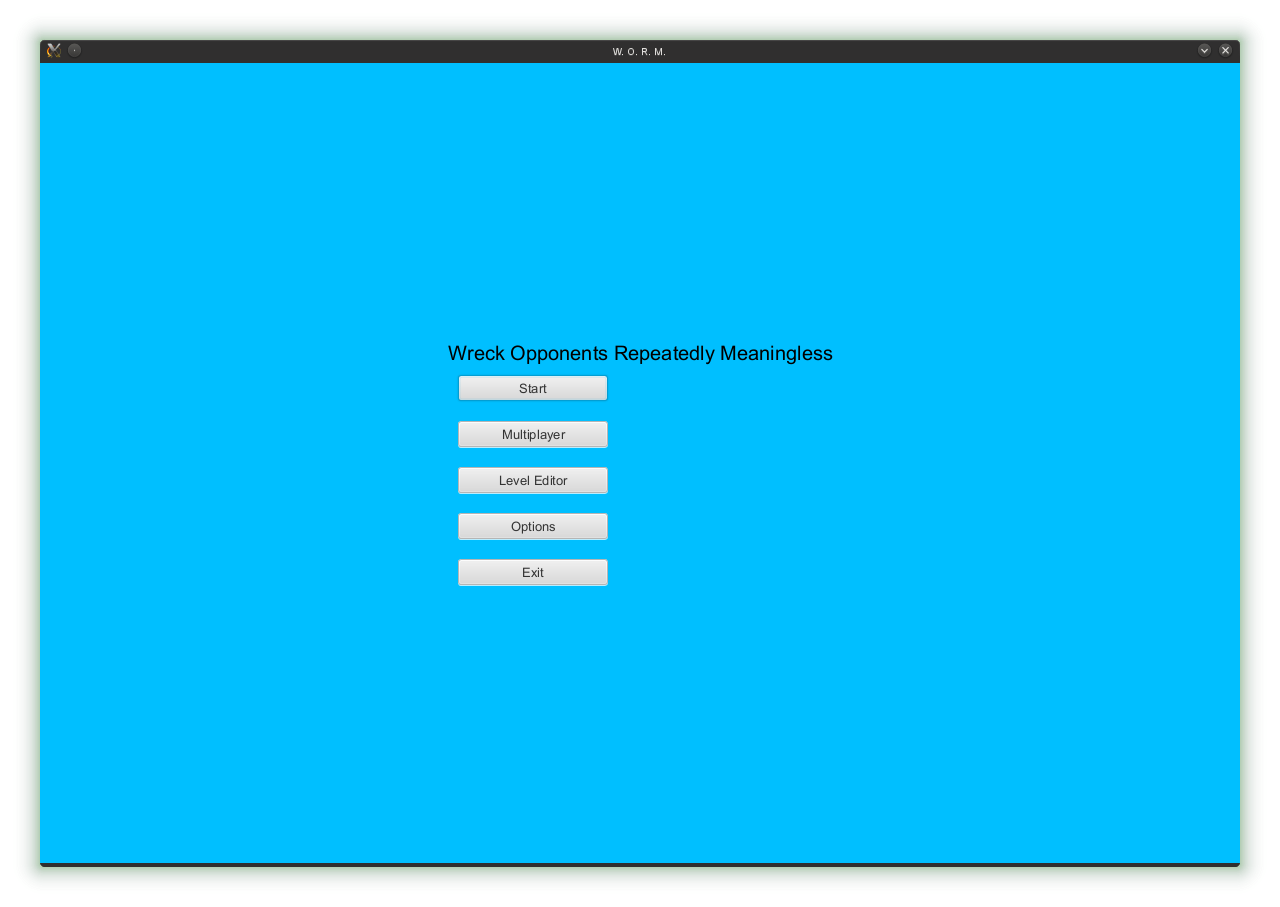
\includegraphics[height=9cm]{Screenshot1.png}

Start – Startet ein lokales Spiel (siehe Kapitel \hyperref[Das Spiel]{ „Das Spiel“})

Multiplayer – Startet ein Netzwerk-Spiel (siehe Kapitel \hyperref[Multiplayer]{„Multiplayer“})

Level Editor – Startet den Modus zum Kreieren eigener Levels (siehe Kapitel \hyperref[Level Editor]{„Level Editor“})

Options – Ermöglicht die Festlegung diverser Einstellungen (siehe Kapitel \hyperref[Optionen]{„Optionen“})

Exit – Beendet das Spiel

\chapter{Das Spiel}
\label{Das Spiel} 
\section{Ein Spiel erstellen}

Durch das Klicken auf den „Start“-Knopf im Hauptmenü gelangt man zu den Spielereinstellungen.

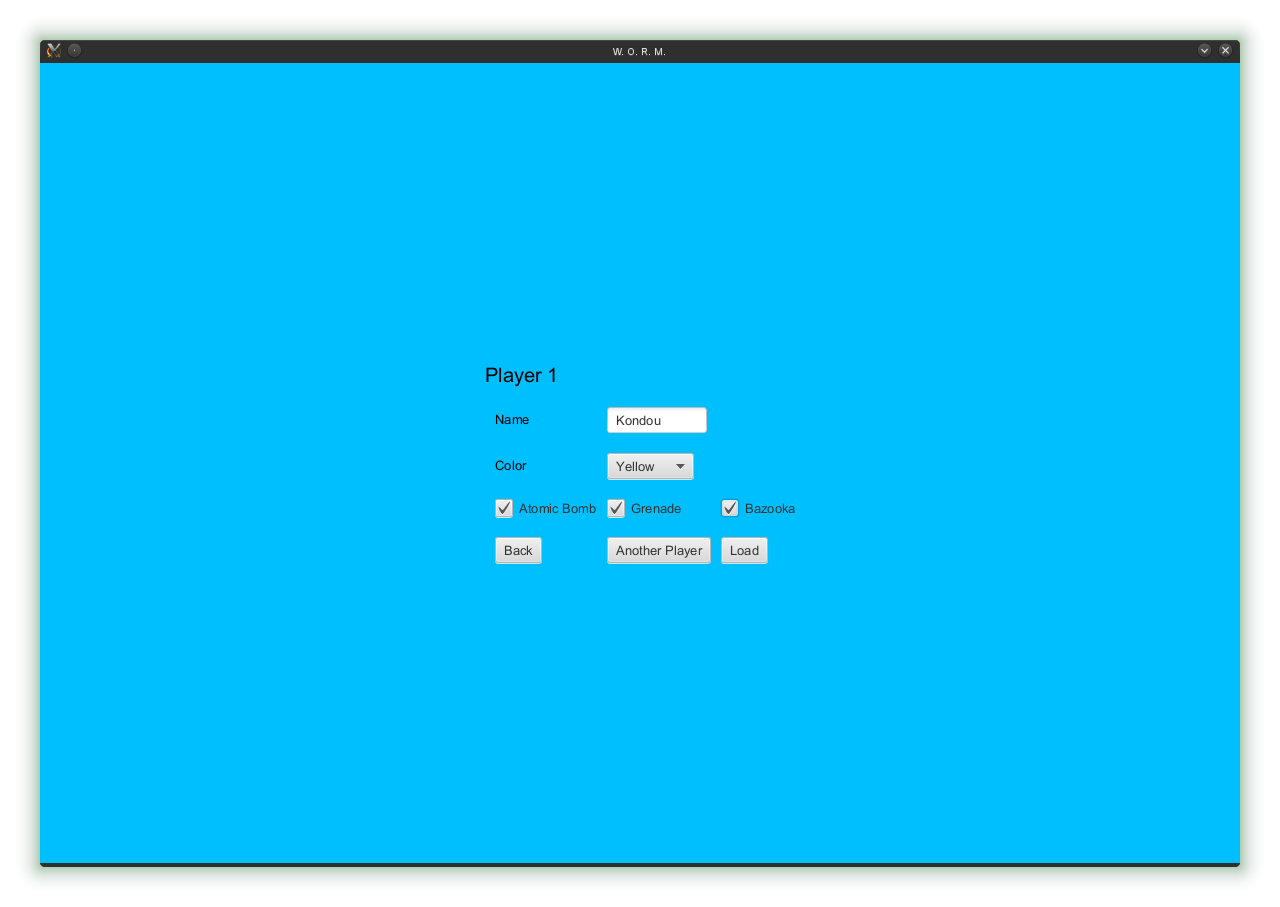
\includegraphics[height=9cm]{Screenshot5.png}

Jeder Spieler hat die Möglichkeit, seinem Team einen Namen zu geben.
Neben der Farbeinstellung ist es zudem notwendig, mindestens eine Waffe auszuwählen, da die Würmer ansonsten keine Waffe zum Angreifen haben.

Alternativ lässt sich über den „Load“-Knopf auch ein zuvor gespeichertes Spiel laden.

Nach der Einstellung des ersten Spielers kann durch das Klicken auf den Knopf „Another Player“ der zweite Spieler sein Team konfigurieren.

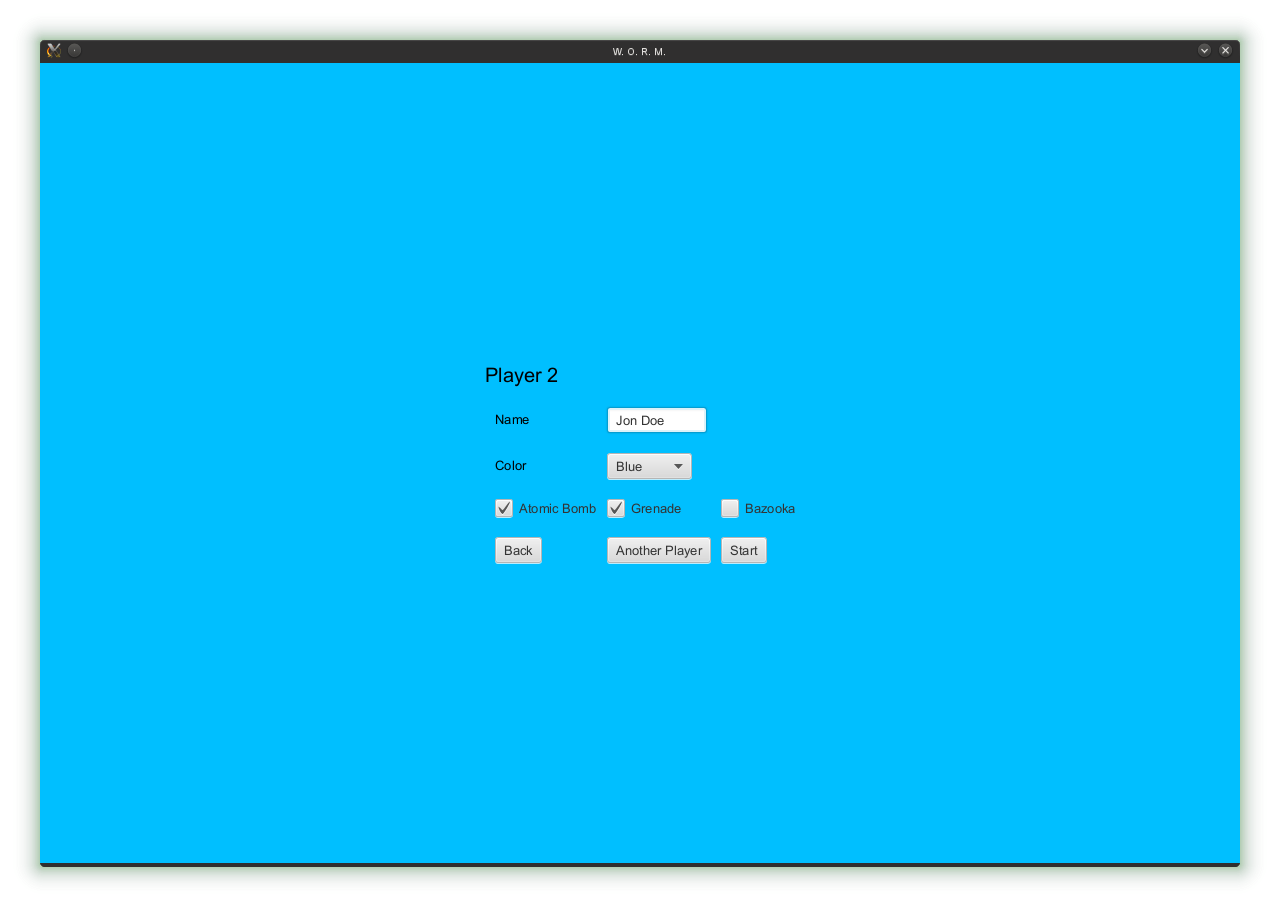
\includegraphics[height=9cm]{Screenshot6.png}

Durch den „Back“-Knopf gelangt man wieder zurück zum Hauptmenü.

Nach der Teamerstellung des zweiten Spielers kann entweder noch ein dritter bzw. vierter Spieler
hinzugefügt werden, oder das Spiel gestartet werden.

Durch das Klicken auf den „Start“-Knopf gelangt man in den Bildschirm zur Levelauswahl, in dem die Mög\-lichkeit
besteht, zwischen verschiedenen Levelkarten zu wählen.

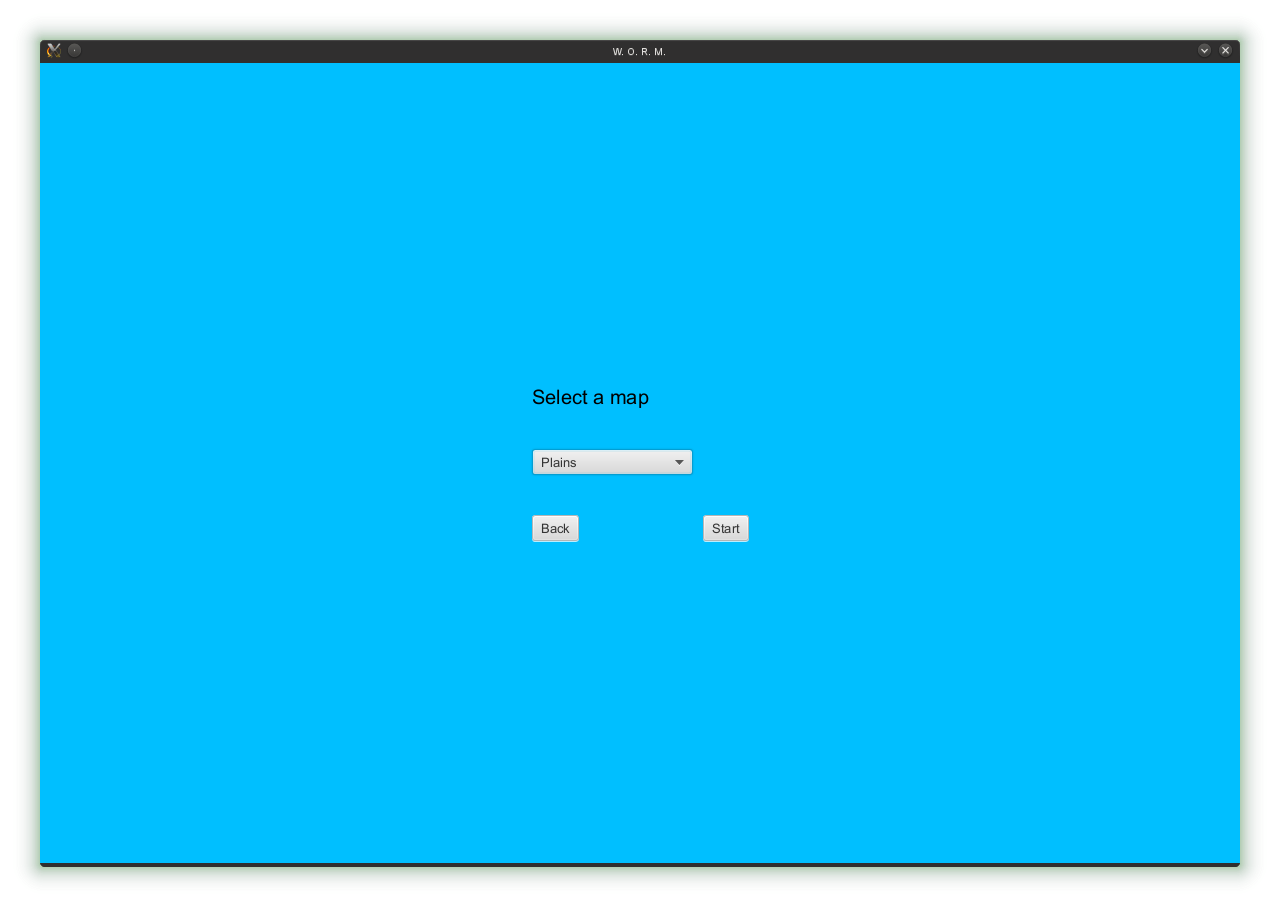
\includegraphics[height=9cm]{Screenshot7.png}

Die Levelkarte Random stellt dabei einen Spezialfall dar, da diese zufallsgeneriert ein Level erstellt.

Klickt man nun auf „Start“, wird das gewählte Level geladen und das eigentliche Spiel gestartet.

\section{Das Spiel}

\subsection{Erläuterung der Oberfläche}

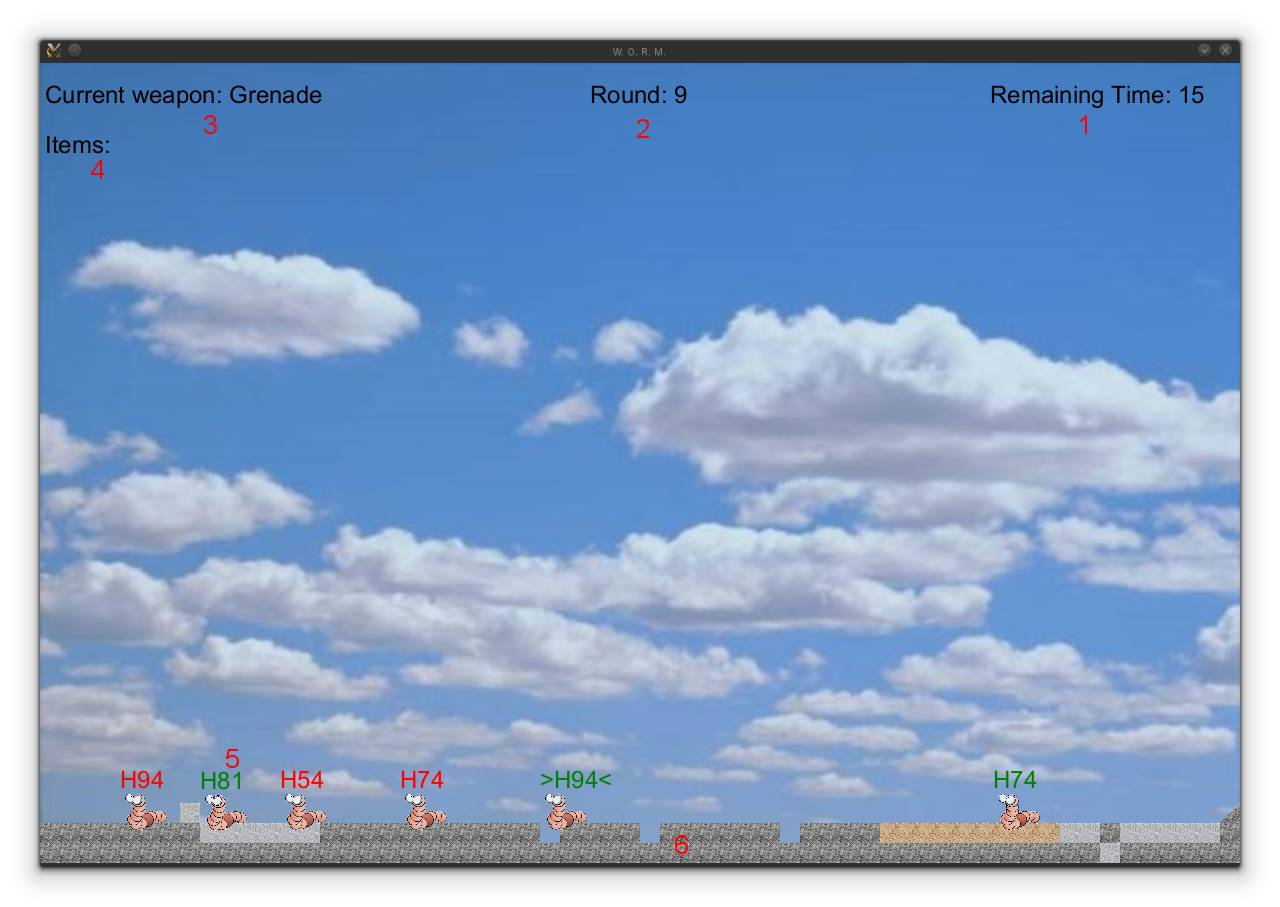
\includegraphics[height=9cm]{Screenshot13.jpg}

\begin{enumerate}
 \item Verbleibende Zeit für die Runde
 \item Zähler, der die aktuelle Runde anzeigt
 \item Aktuell ausgewählte Waffe
 \item Eingesammelte Gegenstände des aktuellen Wurms
 \item Wurm mit Lebenspunkten über seinem Kopf; der mit „\texttt{><}“ eingerahmte Wurm ist aktuell am Zug
 \item Untergrund
\end{enumerate}

\subsection{Bedienung}

\subsubsection{Bewegung}

Durch die Tastaturpfeilknöpfe Rechts und Links bewegen sich die Würmer jeweils nach rechts oder links.

Durch den Tastaturknopf Oben können die Würmen in die vorher ausgewählte Richtung (rechts oder links) springen.

\subsubsection{Schießen}

Die Waffen, die zuvor in den Teameinstellungen festgelegt wurden, werden nun in der oberen linken Ecke des Fensters angezeigt.
Durch Scrollen mit dem Mausrad kann zwischen den Waffen gewechselt werden.

Je nach Position des Mauszeigers können Richtung und Weite des Schusses verändert werden. Dabei gibt die Richtung des Zeigers an, in welche Richtung der Schuss abgefeuert werden soll, während die Entfernung des Zeigers zum Wurm bestimmt, mit welcher Stärke geschossen werden soll.

Durch Klicken der rechten Maustaste wird der Schuss ausgelöst.

\subsubsection{Tastenkürzel}

Während eines Spiels ist es jederzeit möglich, das laufende Spiel auf Druck der „s“-Taste abzuspeichern und mittels der Ladefunktion zu einem späteren Zeitpunkt fortzuführen.
Handelt es sich um ein Netzwerkspiel, kann zudem durch Drücken der „x“-Taste das Spiel synchronisiert werden.

\subsection{Items}

Es gibt 3 verschiedene Gegenstände. Jeder davon kann eingesammelt werden und wird anschließend an der dafür vorgesehenen Stelle oben links im Fenster aufgeführt.
Items werden nummeriert aufgelistet und beim Drücken der jeweiligen Nummer verwendet. 

Elixir: Dieses Item verdoppelt das vorhandene Leben des Wurmes

Schuh: Durch dieses Item können die Würmer schneller auf Sand-Untergrund laufen.

Sprungfeder: Mit diesem Item wird die Sprungkraft des Wurms erhöht.

\subsection{Lebenspunkte}

Jeder Wurm wird durch die Teameinstellung einer Farbe zugeordnet. Die Lebenspunkte über den Würmern werden entsprechend dieser Farben angezeigt.
Jeder Wurm erhält zu Beginn des Spieles 100 Lebenspunkte.

Diese verringert sich, wenn ein Wurm von einem Geschoss getroffen wird oder wenn er von einer großen Höhe fällt.

Ein Wurm ist kampfunfähig, wenn seine Lebenspunkte auf 0 sinken oder er sich in den Bereich außerhalb des angezeigten Spielfeldes bewegt.

\chapter{Multiplayer}
\label{Multiplayer} 

Neben dem lokalen Spielmodus ist es auch mit Hilfe eines Internetservers möglich, mit anderen Spielern über Internet ein Spiel auszutragen.

\section{Eigener Server}

Der Standardserver – schaepers.it - ist für unkomplizierte Online-Spiele nutzbar; jedoch ist auch eine Einrichtung und der Betrieb eines eigenen Servers möglich.

Hierzu startet man die beiliegende „Server.jar“-Datei entweder direkt im Dateibrowser oder in der Kommandozeile mit dem Kommando
\texttt{java -jar Server.jar}.

Zu beachten ist, dass beim Verwenden von Firewalls der  Port 7601 freigegeben sein muss, um Verbindungsprobleme zu vermeiden.

\section{Lobby}

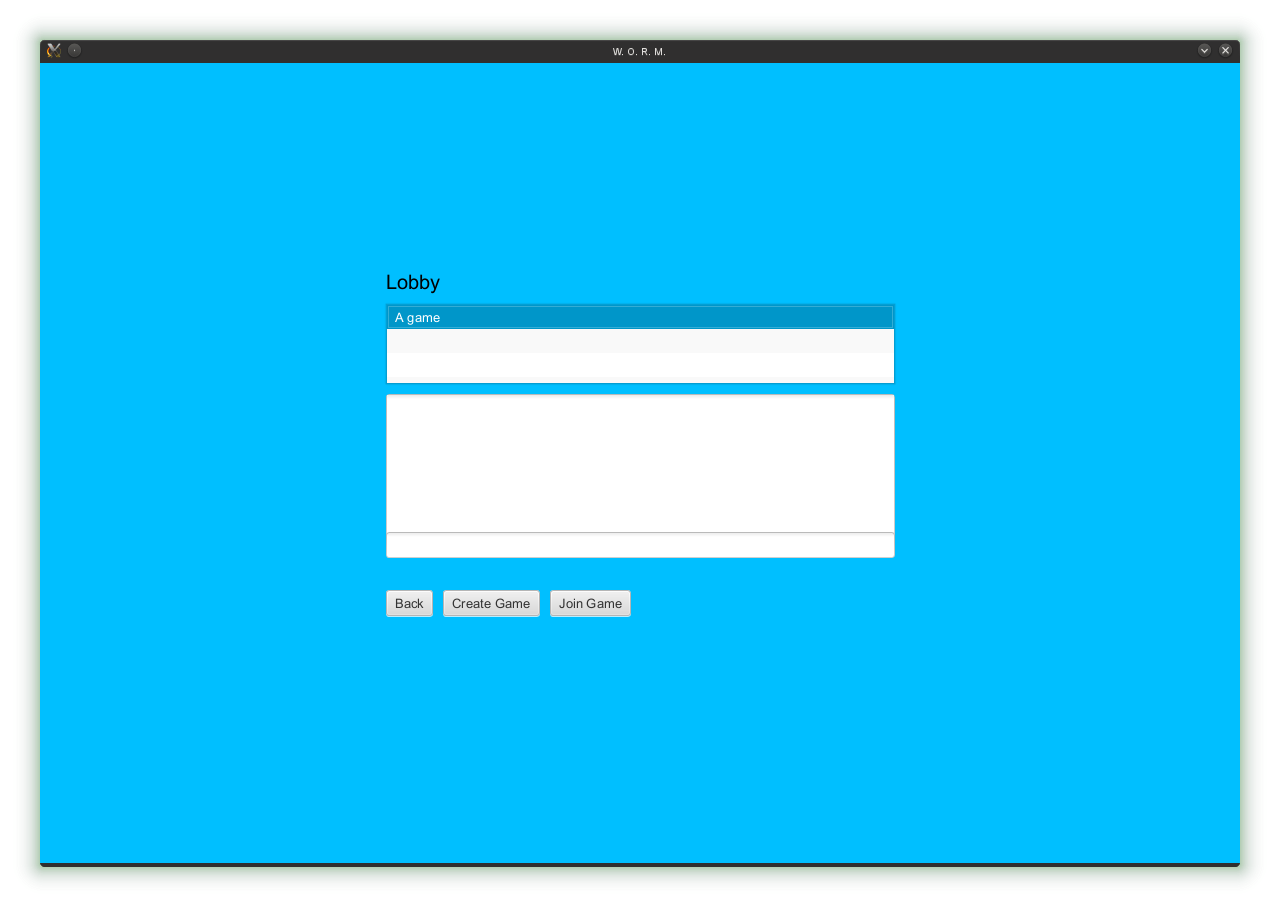
\includegraphics[height=9cm]{Screenshot8.png}

Dies ist der Lobby-Bildschirm; hier kann man entweder mit anderen Spielern auf dem gleichen Server global chatten oder einem
Spiel beitreten.

Mit dem „Back“-Knopf gelangt man zurück ins Hauptmenü.

Mit dem „Create Game“-Knopf kann man einen Raum erstellen (siehe hierzu den Abschnitt \hyperref[Raum]{„Raum erstellen“}).

Mit dem „Join Game“-Knopf kann man dem erstellten Raum eines Spielers beitreten.

\section{Raum}

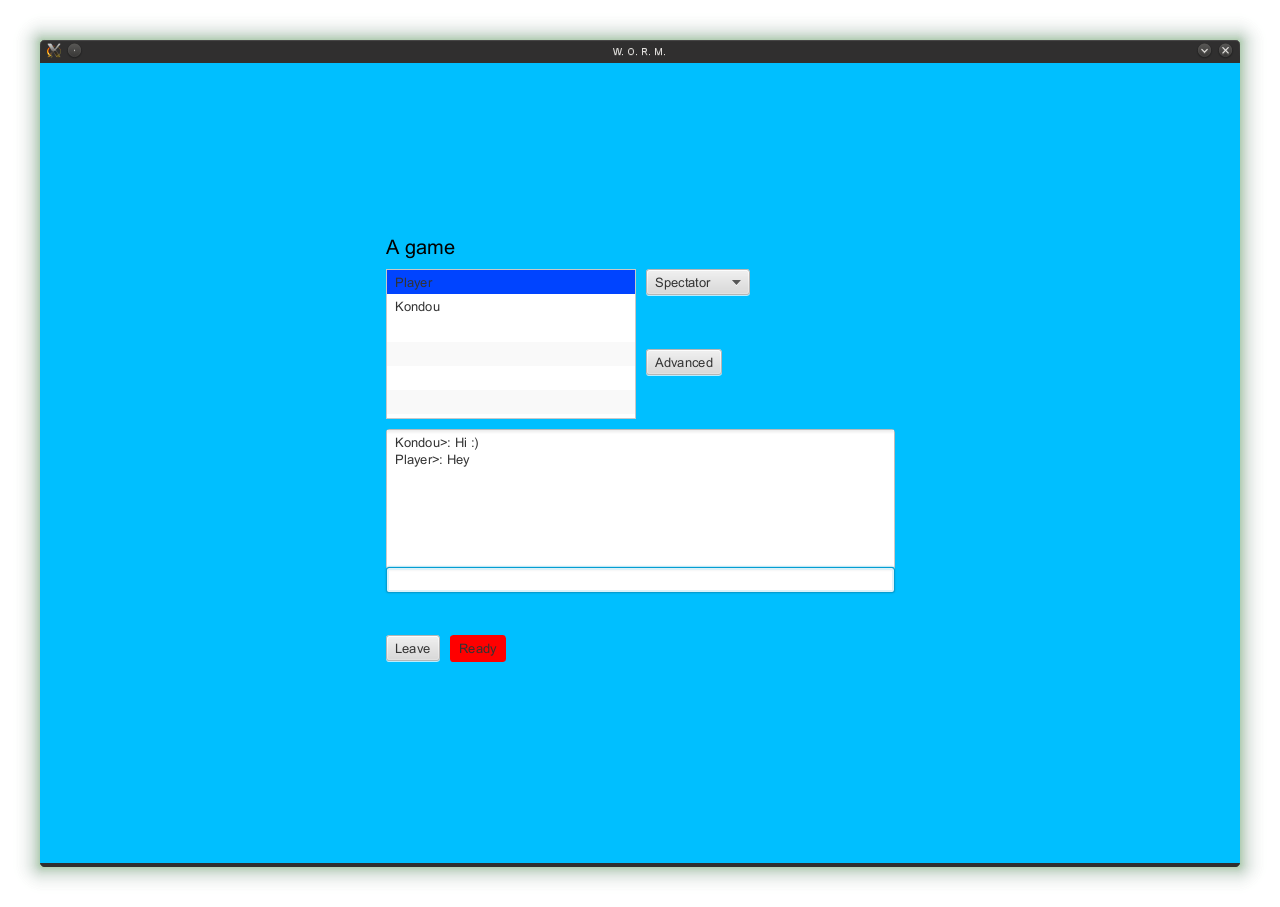
\includegraphics[height=9cm]{Screenshot10.png}

Dies ist der Raum-Bildschirm; hier werden die Spieler mit ihren entsprechenden Team-Farben (bzw. der Farbe Weiß für
Zuschauer) angezeigt. Außerdem besteht die Möglichkeit, mit den Spielern im selben Raum zu chatten.

Mit dem „Leave“-Knopf wird der aktuelle Raum verlassen, um zum Lobby-Bildschirm zurückzukehren.

Mit dem „Ready“-Knopf können Spieler ihre Bereitschaft zum Spielen anzeigen; dabei gibt die Farbe den Status an (Grün steht für „bereit“,
Rot steht für „nicht bereit“).\\
Der Spielleiter verfügt über keinen „Ready“-Knopf, sondern stattdessen einen „Start“-Knopf, welcher das Spiel startet, sobald alle anderen Spieler bereit sind. Die Farbe des Start-Knopfes wird grün, falls alle anderen Spieler bereit zum Spielen sind; ist jedoch auch nur ein Spieler noch nicht bereit, so ist der Knopf rot.

\subsection{Raum erstellen und bearbeiten}
\label{Raum} 

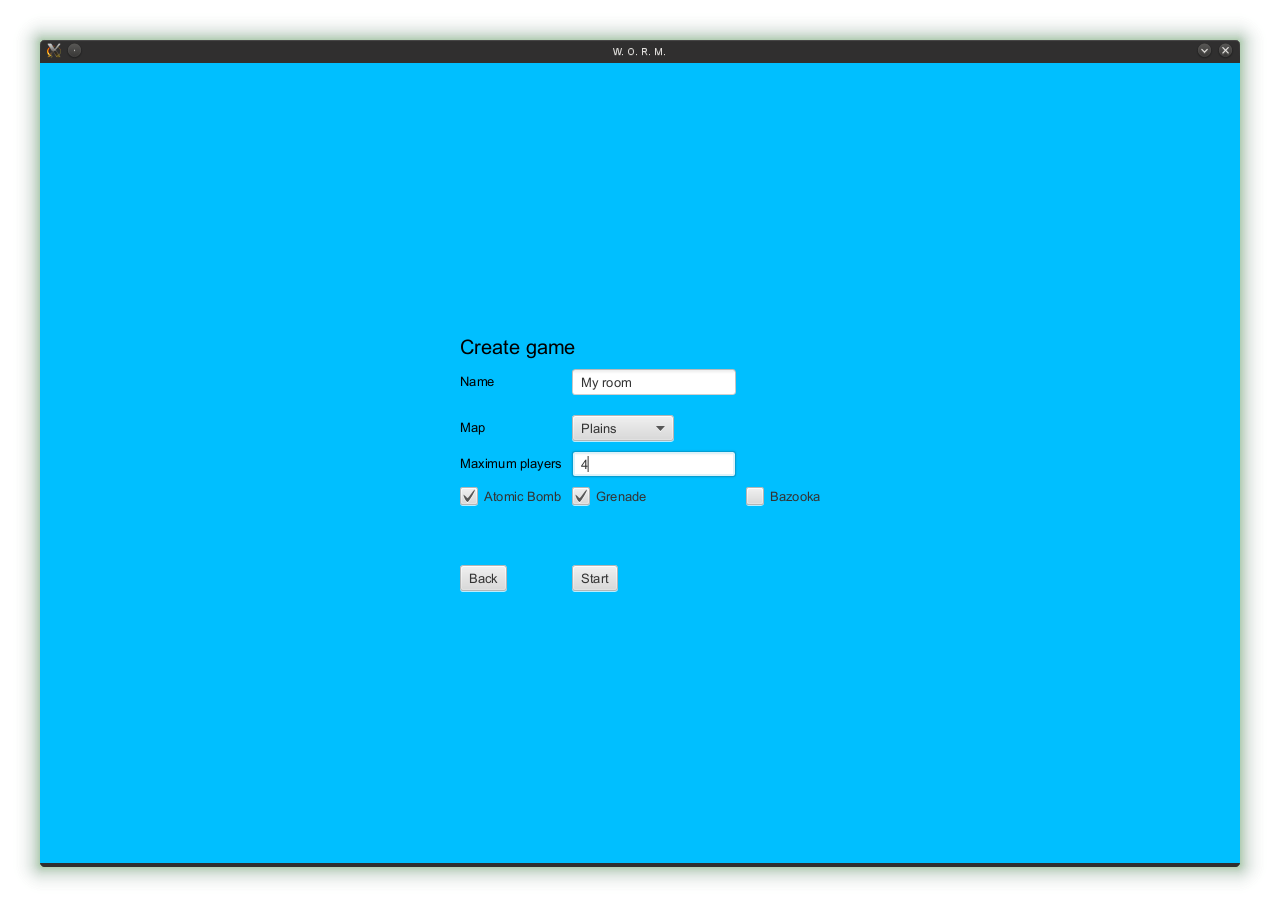
\includegraphics[height=9cm]{Screenshot14.png}

Mit dem „Create Room“-Knopf aus dem Lobby-Bildschirm lässt sich ein Raum erstellen.

Hier lassen sich der Name des Raumes, die zu nutzende Karte, die maximale Anzahl an Spielern und die ausrüstbaren Waffen einstellen.

Mit dem „Start“-Knopf wird die Raumerstellung gemäß der gewählten Einstellungen ausgeführt; mittels des „Back“-Knopfs bricht man diese jedoch ab und gelangt zurück in die Lobby.

Das Bearbeiten eines Raums ist über den „Advanced“-Knopf im Raum-Bildschirm möglich und funktioniert analog zur Erstellung.


\section{Netzwerkspiel}

Das Netzwerkspiel funktioniert ähnlich wie das lokale Spiel, nur dass die teilnehmenden Spieler nicht alle am selben Computer sitzen, sondern über Internet von verschiedenen Rechnern aus miteinander spielen können.

\subsection{Chat}

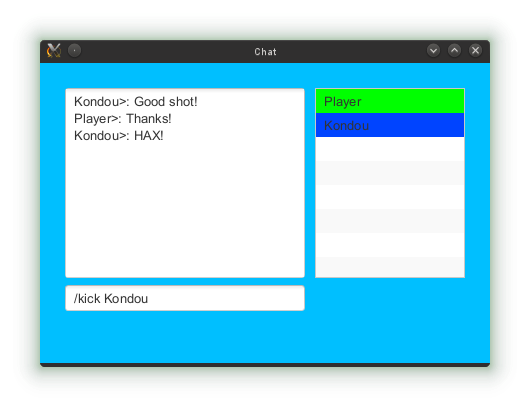
\includegraphics[height=9cm]{Screenshot12.png}

Während eines Netzwerkspiels ist es möglich, per Chat mit den Gegenspielern zu kommunizieren. Der Chat lässt sich auf Wunsch auch schließen oder wieder öffnen.

Der Spielleiter kann außerdem – falls nötig - störende Spieler aus dem Spiel werfen, indem er \texttt{/kick [Spielername]} schreibt und mit Enter
bestätigt.

\chapter{Level Editor}
\label{Level Editor} 

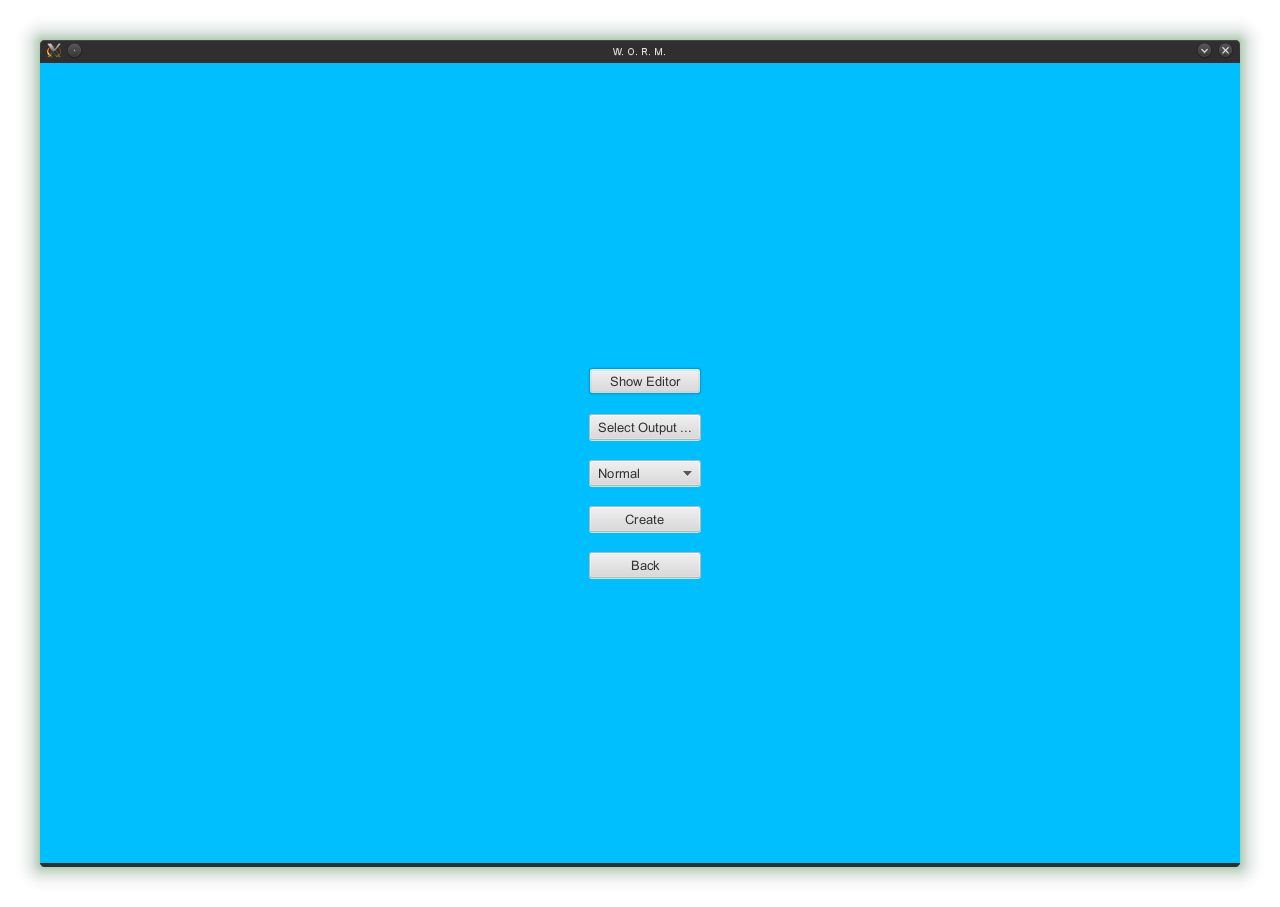
\includegraphics[height=9cm]{Screenshot3.png}

Im Hauptmenü wird durch das Drücken auf den „Level Editor“-Knopf ein Fenster geöffnet, in welchem man ein eigenes Level erstellen kann.

Der Knopf „Show Editor“ wechselt in den Bildschirm, in welchem das Level bearbeitet werden kann. Dabei wird durch mehrfaches Betätigen der linken
Maustaste zwischen verschieden Böden oder Items gewechselt; mit Rechtsklick werden Startpositionen der Würmer festgelegt.

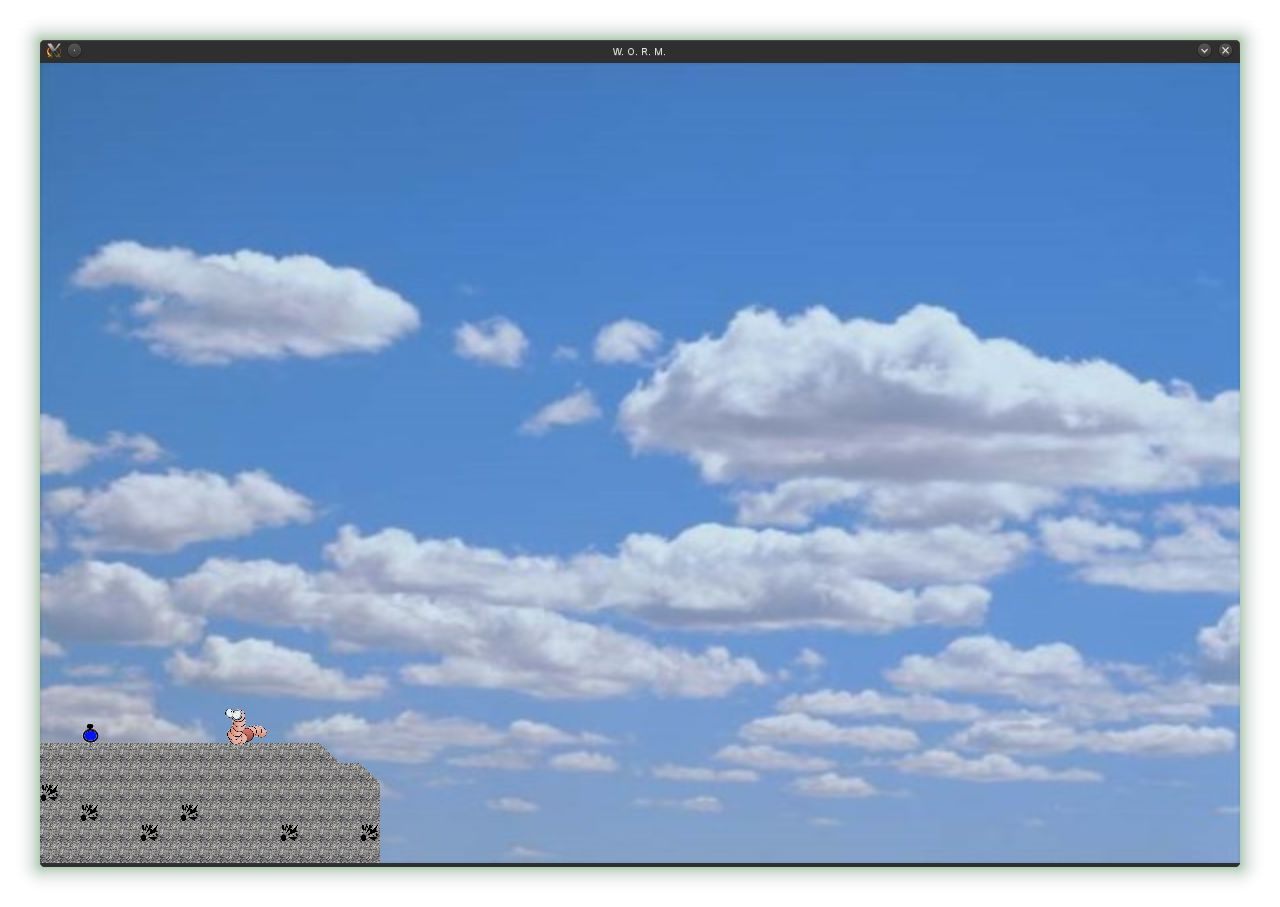
\includegraphics[height=9cm]{Screenshot4.jpg}

Bei Klick auf den „Select Output“-Knopf öffnet sich ein Fenster, in dem ausgewählt werden kann, wo genau das erstellte Level abgespeichert werden soll. Es wird empfohlen, selbsterstelle Karten im entsprechenden Verzeichnis \texttt{maps} zu speichern, da Karten in diesem Verzeichnis vom Programm erkannt werden und dann bei der Kartenauswahl zur Verfügung stehen.

In der Dropdown-Liste unter dem „Select Output“-Knopf lassen sich die unterschiedlichen Themen Normal, Horror und Oriental auswählen, von denen abhängt, welches Hintergrundbild angezeigt und welche Hintergrundmusik im Level abgespielt werden wird.

Durch Drücken des „Create“-Knopfs wird das erstellte Level unter dem oben angegebenen Pfad mit dem gewählten Thema abgespeichert.

Mit dem Knopf „ Back“-Knopf wird wieder zurück ins Hauptmenü gewechselt.

\chapter{Optionen}
\label{Optionen} 

Klickt man auf „Optionen“, wird in ein Fenster mit verschiedenen Einstellungen gewechselt.

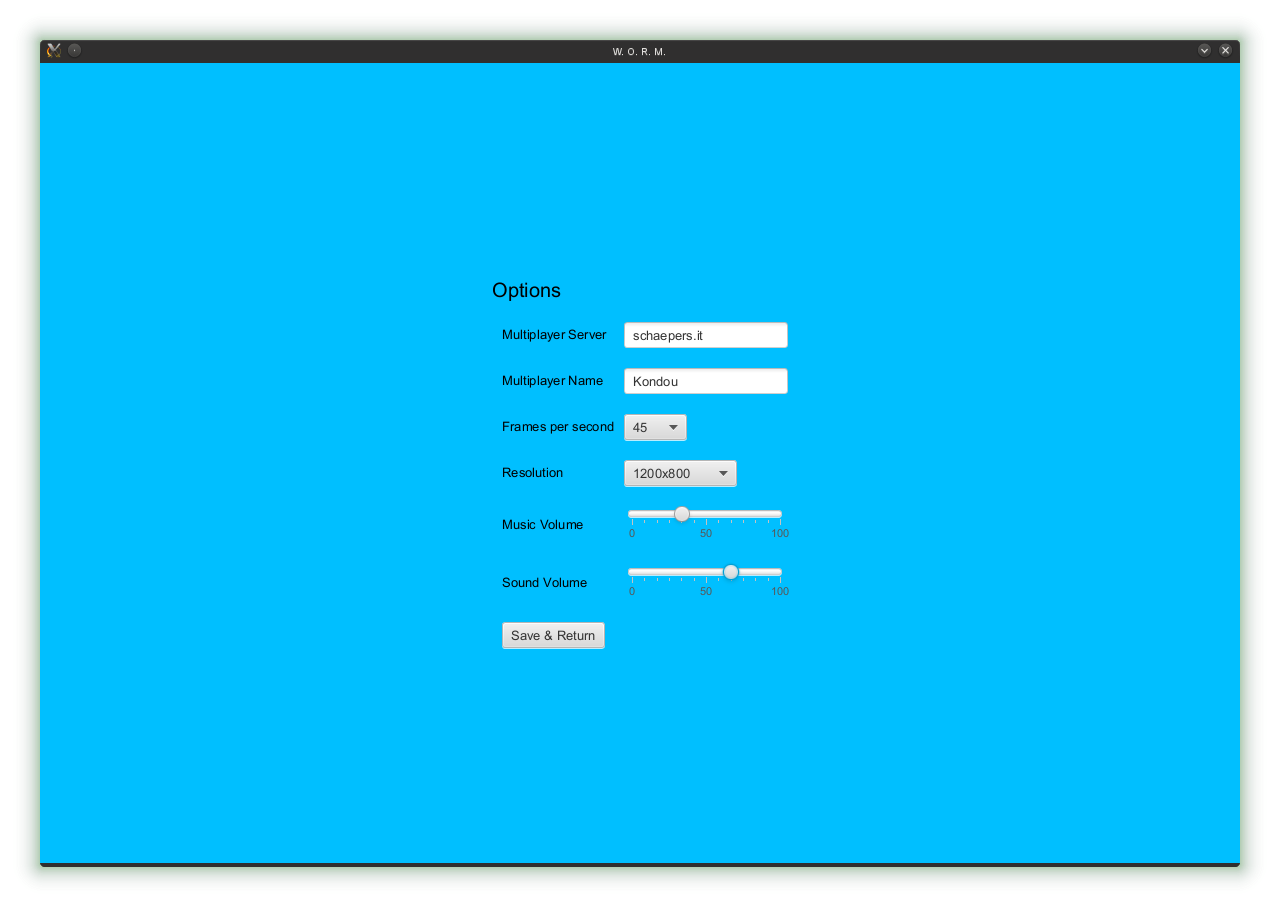
\includegraphics[height=9cm]{Screenshot2.png}

\underline{Multiplayer Server}\\
Hier lässt sich einstellen, mit welchem Server man sich für Netzwerkspiele verbindet. Der Standard-Server ist der von
Christopher Schäpers angebotene und unter der Domäne schaepers.it erreichbar.

\underline{Multiplayer Name}\\
Hier lässt sich der eigene Anzeigename für Netzwerkspiele einstellen. Diese Option empfiehlt sich sehr zur Unterscheidung von anderen Spielern, da standardmäßig jeder Spieler den Namen „Worms-Player“ trägt.

\underline{Resolution}\\
Diese Option stellt die Auflösung des Fensters ein. Erst nach Speichern der Einstellungen wird diese angewandt.

\underline{Music-Volume}\\
Dieser Slider ändert die Lautstärke der Hintergrundmusik sowohl im Menü als auch während eines Spiels. Zieht man den Slider nach links, so verringert sich die Lautstärke – umgekehrt erhöht sich die Lautstärke, wenn der Slider nach rechts geschoben wird.

\underline{Sound-Volume}\\
Dieser Slider ändert, analog zu Music-Volume, die Lautstärke der Geräuscheffekte, die z.B. beim Abfeuern von Waffen oder beim Treffen
der Würmer abgespielt werden.

Mit einem Klick auf „Save \& Return“ werden die aktuellen Einstellungen gespeichert und angewandt; anschließend wird zurück ins Hauptmenü gewechselt.

\end{document}
